We evaluate our work using three metrics: performance, scalability and security. For performance evaluation, we measure the impact on performance due to extended KASLR -- caused by position independent code (Section~\ref{sec:eval:pic}) -- as well as from continuous re-randomization (Section~\ref{sec:eval:rand}). We measure the performance penalty due to position independent code by conducting experiments with the file system module compiled as PIC. For re-randomization, we focus on two class of drivers: Ethernet and NVMe. For each of these drivers, we measure the throughput and CPU utilization for various re-randomization periods.

\section{Experimental Setup}
\begin{table*}
\caption{Server and Client systems.}
\begin{center}
\begin{tabular}{ l l l }
\toprule
 & \textbf{Server (System for Evaluation)} & \textbf{Client (Load Generator)} \\
\midrule
CPU & 2 x Intel Xeon Silver 4114, 2.20GHz & 1 x Intel Core i7 4770, 3.40GHz \\
Cores & 10 per CPU & 4 per CPU \\
HyperThreading & OFF (2 per core) & ON (2 per core) \\
TurboBoost & OFF & OFF \\
L1/L2 cache & 64 KB / 1024 KB per core & 64 KB / 256 KB per core \\
L3 cache & 14080 KB & 8192 KB \\
Main Memory & 96 GB & 16 GB \\
Network & Intel E1000E 1GbE adapter & Intel E1000E 1GbE adapter \\
Storage & Samsung 970 EVO NVMe & Samsung 860 EVO SSD\\
\bottomrule
\end{tabular}
\end{center}
\label{tbl:system}
\end{table*}

In all of our tests we used Ubuntu 18.04. We updated the Linux kernel to a newer version of v5.0.2. The server runs Ubuntu Server whereas the client machine runs the Ubuntu Desktop. Table~\ref{tbl:system} shows our hardware specifications. The machines run all the default packages that come with Ubuntu in addition to other packages such as the Apache server, MySQL server, SysBench~\cite{web:sysbench} and ApacheBench~\cite{APACHEBENCH} that were used for the experiments.
To compare the performances, we generated different test kernel combinations from the default Ubuntu configuration by toggling the following features:
\begin{itemize}[noitemsep]
\item Retpoline (Spectre mitigation patch)
\item Position Independent Modules
\item Stack Re-Randomization
\item Module Address Space Re-Randomization
\end{itemize}

All of the generated configurations compile over 5000 kernel modules.

We ran all of our experiments for ample duration of time yielding a low standard deviation. Each experiment was conducted 3 to 5 times, arithmetic mean was plotted along with error bars showing the standard deviation from mean (where applicable).

\section{Position Independent Modules}
\label{sec:eval:pic}
\begin{figure}[ht!]
\centering
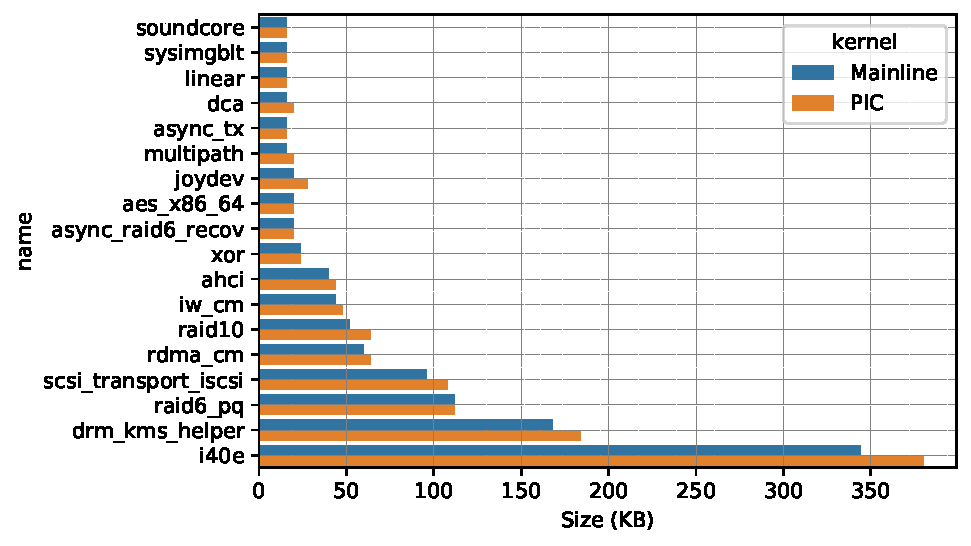
\includegraphics[width=0.7\columnwidth]{charts/module_sizes.pdf}
\caption{Module size (PIC vs. non-PIC), KB}
\label{fig:modulesiszes}
\end{figure}

We first conducted various experiments to test position-independent modules (our first contribution), their overall impact on system performance, and memory footprint.

In Figure~\ref{fig:modulesiszes}, we randomly selected twenty modules to demonstrate the difference in memory footprint resulting from position-independent (PIC) model.
We found the difference in memory footprint of retpoline and non-retpoline cases to be insignificant; thus, we only present the position-independent and the mainline Linux modules with retpoline enabled. Our analysis show that PIC causes an increase in memory footprint of about 10 \%.

Next we ran several micro- and macro- benchmarks to evaluate the performance impact of PIC modules. We evaluated four Linux configurations:
\begin{enumerate}[noitemsep]
    \item Mainline Linux without retpoline
    \item Mainline with retpoline
    \item Our PIC changes without retpoline
    \item Our PIC changes with retpoline
\end{enumerate}
We used the default Ubuntu configuration in all tests. Since we performed some file system tests, we also
compiled the \verb|ext4| Linux filesystem driver as a module.

\begin{figure}[ht!]
\centering
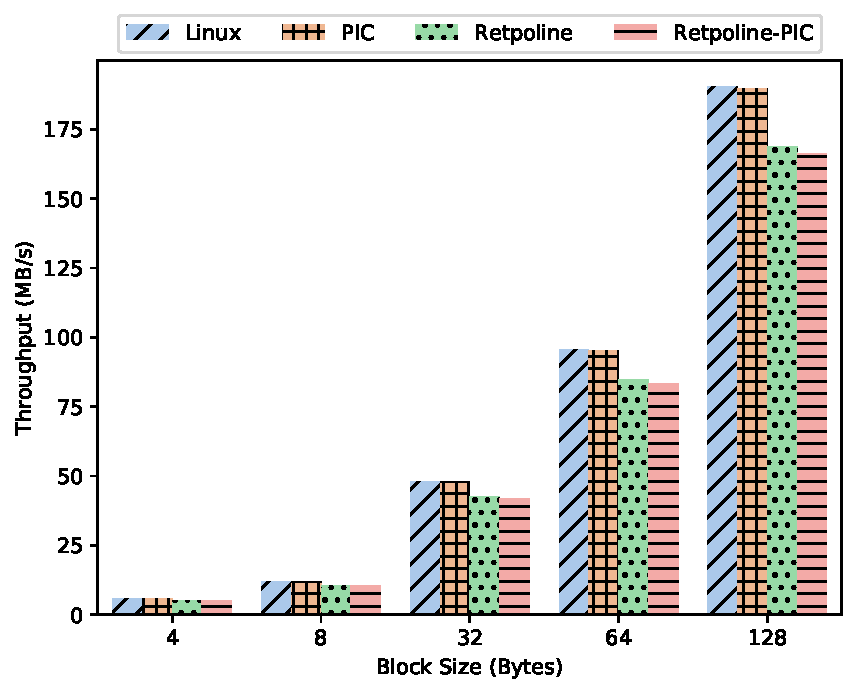
\includegraphics[width=0.7\columnwidth]{charts/file_micro.pdf}
\caption{Filesystem Microbenchmark}
\label{fig:file_micro}
\end{figure}

Figure~\ref{fig:file_micro} shows the results of our own micro-benchmark which uses \verb|dd| to read files with varying block sizes. This test is CPU bound due to the use of the buffer cache. This experiment revealed the real impact of retpoline (Spectre mitigation patches). Figure \ref{fig:file_micro} shows that without retpoline the performance of PIC and non-PIC is nearly the same. There is some performance penalty introduced by the PIC code when retpoline is enabled. This slight performance degradation is caused by the need of \verb|retpoline safe| indirect jumps to external functions in \verb|PLT| stubs of the position independent code.

We used  the \verb|sysbench file_io| benchmark to measure the throughput on random and sequential reads. For this experiment, the files were also cached in RAM to keep the results I/O invariant. The results in Figure~\ref{fig:sysbench_file} show that the performance of PIC-enabled systems is identical to their non-PIC counterparts.

\begin{figure}[ht!]
\centering
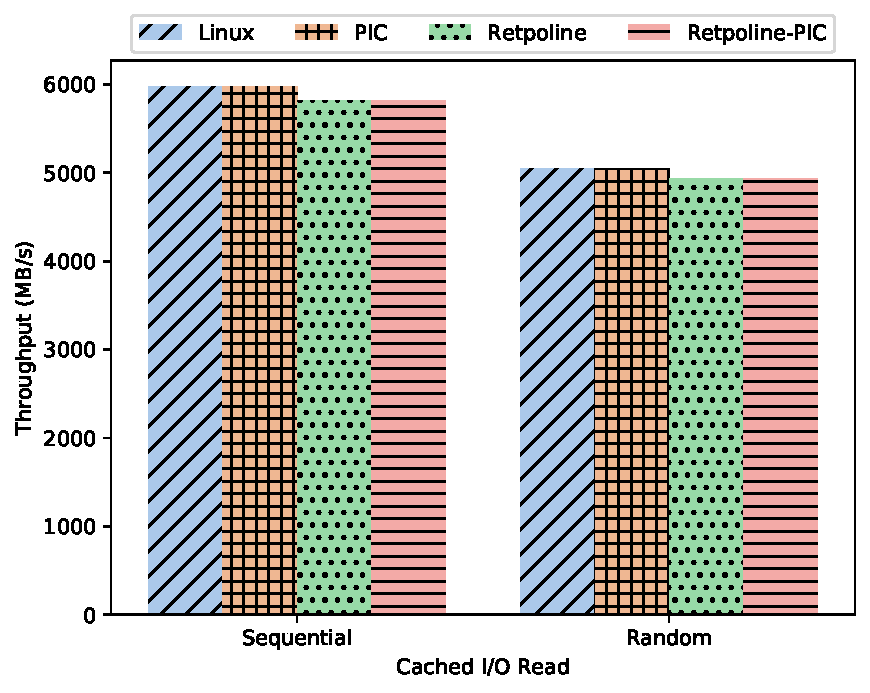
\includegraphics[width=0.7\columnwidth]{charts/sysbench_io.pdf}
\caption{Sysbench Filesystem (Cached)}
\label{fig:sysbench_file}
\end{figure}

\verb|Kernbench| is a CPU throughput benchmark that is often used to compare kernels. We recorded system time (time spent in kernel space) at 3 levels of concurrency. The results as reported in Figure~\ref{fig:kernbench} show that PIC modules have insignificant performance impact.

\begin{figure}[ht!]
\centering
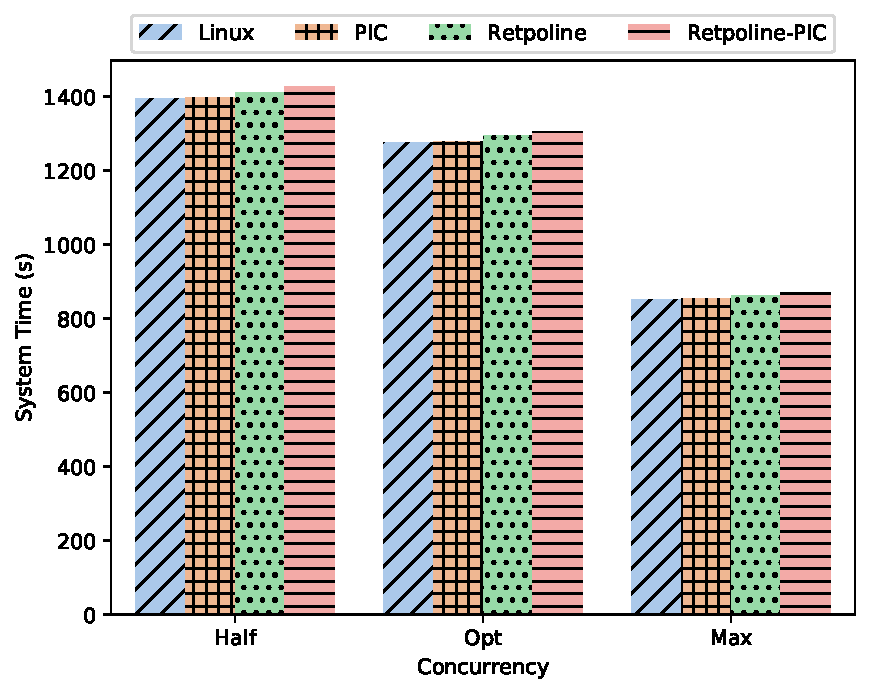
\includegraphics[width=0.7\columnwidth]{charts/kernbench.pdf}
\caption{Kernbench}
\label{fig:kernbench}
\end{figure}

Our tests show that when retpoline is disabled the PIC code performs just the same as its non-PIC counterpart. In the case when retpoline is enabled, PIC code causes slight performance degradation which is almost negligible. Since the effect of retpoline is insignificant, in the later sections we limit the comparison of our work to mainline Linux compiled with retpoline enabled.

\section{Re-Randomization}
\label{sec:eval:rand}
There is currently no continuous re-randomization solution available for the Linux kernel. Therefore, we compare our implementation directly with vanilla Linux. In this report, we evaluate two classes of randomized drivers. First, we evaluate the \verb|e1000e| network driver, which is a popular Intel's Ethernet driver. Then we evaluate the \verb|NVM Express block device| driver that is used for NVMe solid state drives.

\subsection{Network Driver Re-Randomization}
To evaluate network driver re-randomization, we use Apache and mySQL server installations with default Ubuntu configurations. We ran the corresponding macro-benchmarks from a client machine which is directly connected to the network adapter of our test box (server).

In Figure~\ref{fig:network}, we present results for continuous module re-randomization for different block sizes (512B, 1KB, 4KB and 16KB). Smaller block sizes typically put more stress on the system as the total number of system calls increases. We set different re-randomization intervals (1 and 5 ms) and compare against mainline Linux. We present CPU usage across all CPUs.
As Figure~\ref{fig:network} shows, re-randomization does not impact overall system throughput even for high concurrency. Re-randomization does result is slightly elevated CPU usage ($\approx 2 \%$ for 1 ms); the additional CPU usage is independent of the network load and concurrency.

\begin{figure}[ht!]
\centering
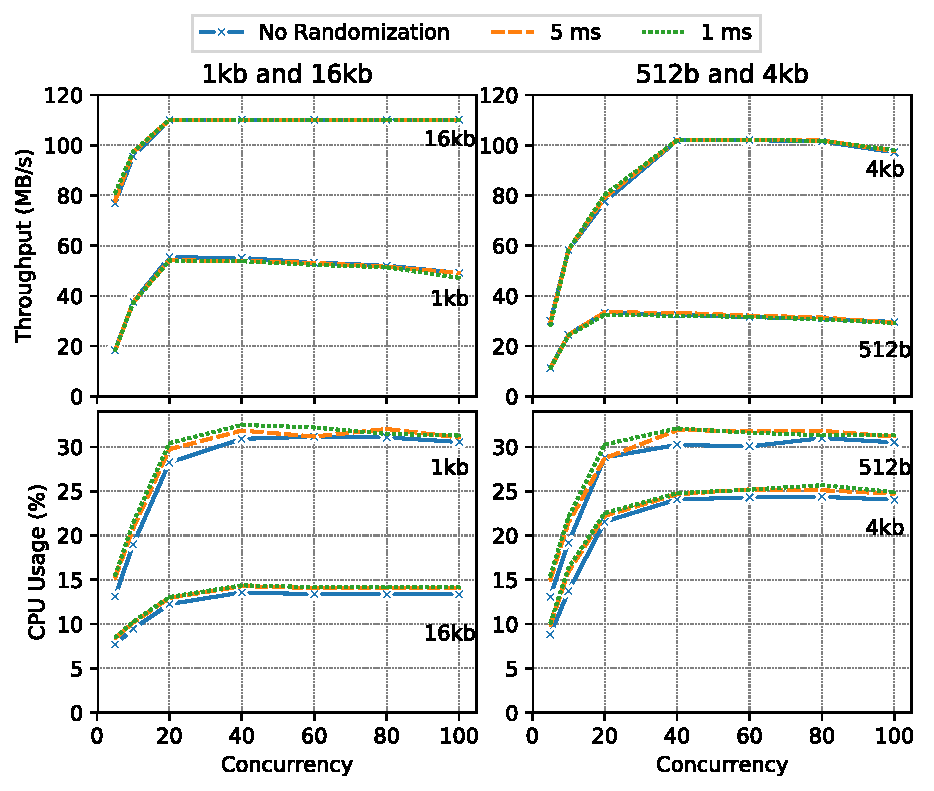
\includegraphics[width=0.8\columnwidth]{charts/apache.pdf}
\caption{ApacheBench: module re-randomization}
\label{fig:network}
\end{figure}

We also measured \verb|mySQL| performance using \verb|sysbench| \verb|oltp| on a database comprising of 10 tables with 1,000,000 rows of data each. The database was cached in memory and the experiment was conducted with varying levels of concurrency and different re-randomization periods. The rate of transactions was measured along with network throughput and CPU utilization, and the results are shown in Figure~\ref{fig:sysbench_sql}. The graphs show that the database performance is unaffected by a re-randomization period and the additional CPU utilization is independent of the system load.

\begin{figure}[ht!]
\centering
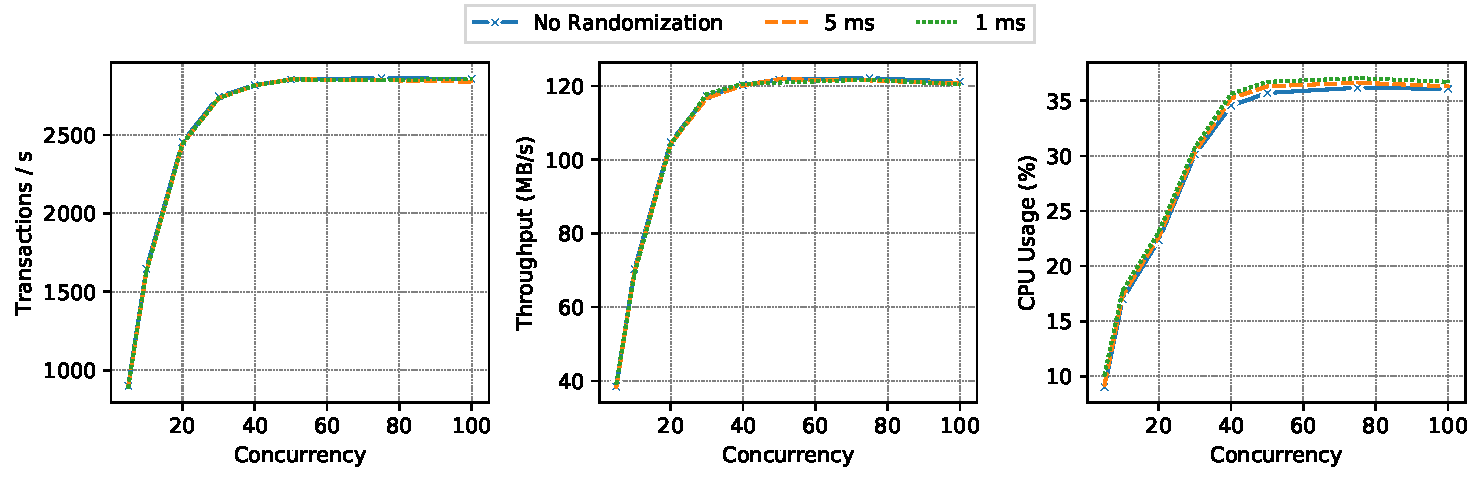
\includegraphics[width=\columnwidth]{charts/sysbench_sql.pdf}
\caption{Sysbench OLTP}
\label{fig:sysbench_sql}
\end{figure}

\subsection{NVMe Driver Re-Randomization}
In order to reliably measure the performance of the NVMe driver under re-randomization, it was important to design an experiment that minimizes the effects of I/O in the underlying hardware. We created our own benchmark that measures the read throughput of a file stored on the NVMe storage. The file is opened with \verb|O_DIRECT| and \verb|O_SYNC| flags using the \verb|open()| syscall, and a block (of 512 bytes) is repeatedly read from the start of the file in a tight loop. The \verb|O_DIRECT| and \verb|O_SYNC| flags guarantee synchronous data transfer and thus prevent caching of the file by the file-system. We read the same block over and over again to leverage the NVMe's internal DRAM cache in an effort to minimize the I/O wait time and make the benchmark CPU bound.

\begin{figure}[ht!]
\centering
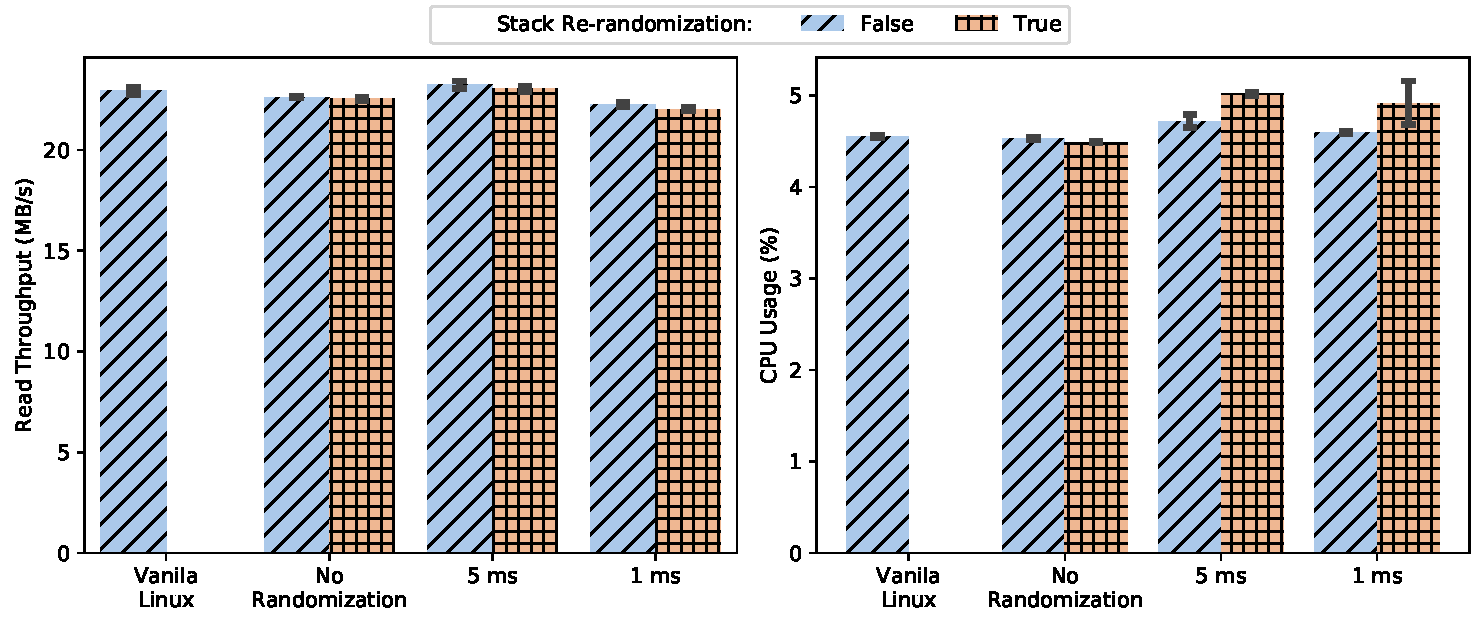
\includegraphics[width=\columnwidth]{charts/nvme_read.pdf}
\caption{NVME Read Throughput}
\label{fig:nvme_read}
\end{figure}

We measured the read throughput of the NVMe drive and recorded the CPU utilization for the duration of the experiment. The results are shown in Figure~\ref{fig:nvme_read}. Apart from the slight increase in CPU utilization, the performance of NVMe storage remains largely unaffected by re-randomization.

\subsection{IOCTL Re-Randomization}
All of our experiments on real-life device drivers showed that re-randomization does not impact the device performance. This can be attributed to the fact that device drivers are I/O bound. The I/O wait time of the device drivers outweighs the CPU time by a large margin and thus the I/O performance penalty due to increased CPU time is minimized. We tested the extreme case of a CPU bounded device driver by designing our own micro-benchmark.

\begin{figure}[ht!]
\centering
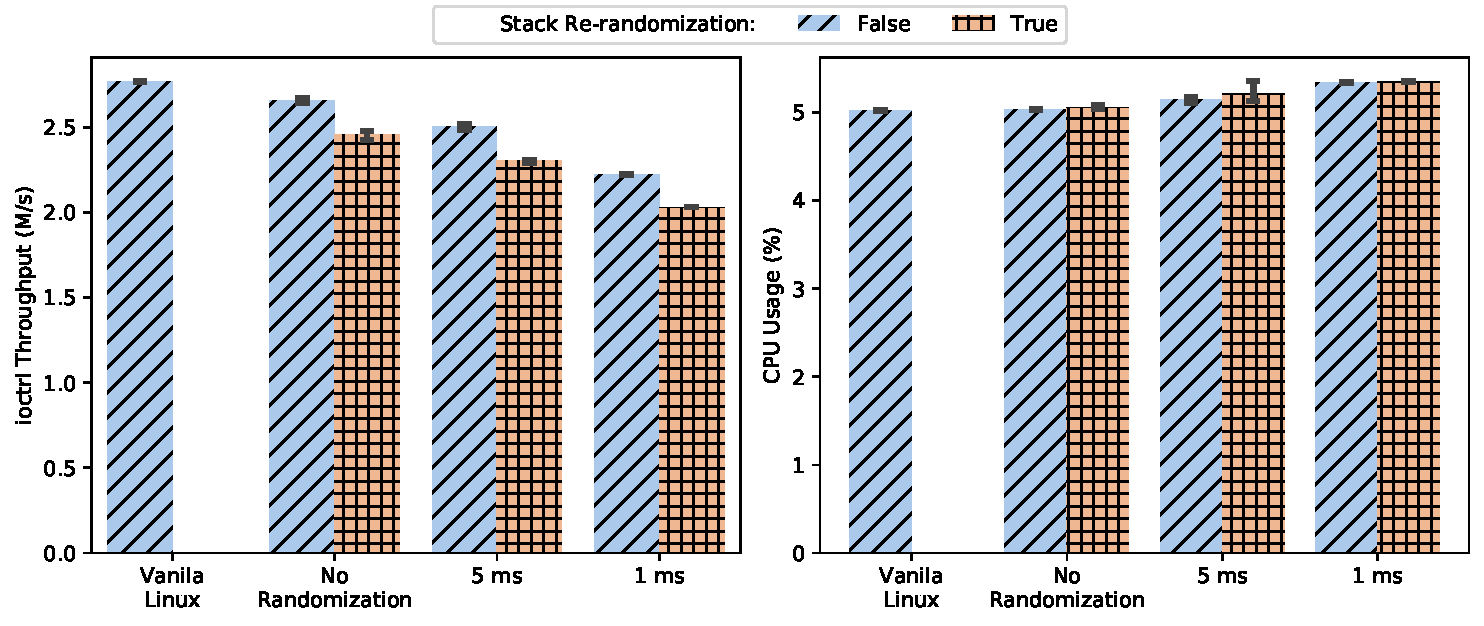
\includegraphics[width=\columnwidth]{charts/ioctrl.pdf}
\caption{IOCTL Throughput}
\label{fig:ioctl}
\end{figure}

We created a dummy device driver that implements a simple \verb|ioctl| operation that just increments the \verb|int| pointer argument passed to it. We repeatedly make the \verb|ioctl()| syscall on the driver in a tight loop and measure the number of ioctl operations performed per second. Figure~\ref{fig:ioctl} shows the ioctl throughput (in million operations per second) along with the corresponding CPU utilization. This benchmark is CPU bound and captures the impact of function wrappers and stack randomization on CPU intensive device operations. It is found that introduction of function wrappers causes a performance drop of $\approx$4\% and stack randomization causes an additional drop of $\approx$6\% when compared to vanilla Linux.

\section{Scalability Analysis}
\begin{wrapfigure}{R}{0.5\columnwidth}
\caption{Re-Randomization Breakdown}
\label{fig:rand_profile}
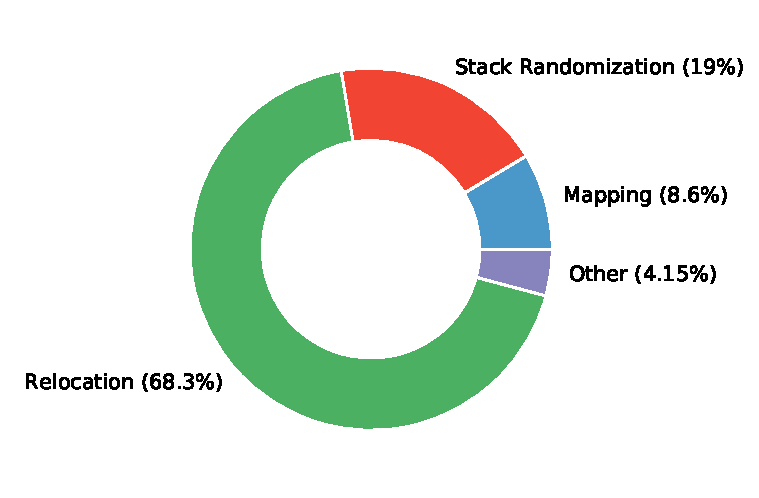
\includegraphics[width=0.5\columnwidth]{charts/rand_profile.pdf}
\end{wrapfigure}

We measured the CPU utilization of the randomization thread to be $0.4\%$ for a randomization period of 20 ms. The breakdown of the CPU utilization is shown in Figure~\ref{fig:rand_profile}. The \textit{stack randomization} and \textit{other} cost is a one-time cost of randomization, independent of the number of modules being randomized. The \textit{virtual page remapping} cost is proportional to the size of the module.

The \textit{relocation} cost is a function of relocation entries in the module object file. Although the re-randomization process only needs to re-apply a fraction of the total relocations in the object file, it has to iterate over all the entries to identify the relevant relocations. We believe with appropriate compiler modifications, the required relocations could be grouped together which would substantially cut down this cost.

A typical server has average utilization of about 20 to 30\%~\cite{bohrer2002case,33387}. With the default Ubuntu configuration, a typical system would use around 100 modules. With 0.32\% CPU utilization per module, our randomization approach can comfortably re-randomize over 150 modules without impacting system performance.

% ============================================================
% ============================================================
% ============================================================

\section{Security Analysis}\label{se:eval_security}
\subsection{Distribution and Availability of ROP gadgets}
In order to gauge the threat posed by ROP gadgets in Linux kernel and to determine the efficacy of our re-randomization approach we used the metrics provided by Follner, et al.~\cite{follner2016analyzing}. We measure the quantity and quality of gadgets in the Linux kernel and its modules. We used Ropper~\cite{schirra_2019}, an ROP gadget finding tool. Ropper can read ELF files, find ROP gadgets and build chains. We studied the ROP gadgets present in Ubuntu 18.04 with default configuration classified under the following three classes:

\begin{enumerate}[noitemsep]
    \item Core Linux kernel
    \item Vanilla modules
    \item PIC modules
\end{enumerate}

Follner, et al.~\cite{follner2016analyzing} proposes two metrics to measure the quantity and quality of ROP gadgets. The first metric is calculated by counting the number of gadgets belonging to twelve proposed categories of operations (Table~\ref{tbl:gadget_categories}). This metric provides information on the quantity of gadgets and is helpful in comparing the number of gadgets between transformed binaries (for example regular modules and PIC modules). The second metric assigns a quality score to an ROP chain based on pre-conditions and side-effects on other registers or memory that a gadget in the chain might have. In our analysis we measure the first metric exactly as proposed by Follner. However, we employ a simplified version of the second metric: we only track if an ROP chain can be constructed with/without side-effects or not.

\newcolumntype{L}{>{\raggedright\arraybackslash}m{12cm}}
\begin{table*}
    \caption{Gadget Categories}
    \begin{center}
    \begin{tabular}{lL}
    \toprule
    \textbf{Category} & \textbf{Included Instructions} \\
    \midrule
    Data move & pop, push, mov, xchg, lea, cmov, movabs \\
    \hline
    Arithmetic & add, sub, inc, dec, sbb, adc, mul, div, imul, idiv, xor, neg, not \\
    \hline
    Logic & cmp, and, or, test \\
    \hline
    Control flow & call, sysenter, enter, int, jmp, je, jne, jo, jp, js, lcall, ljmp, jg, jge, ja, jae, jb, jbe, jl, jle, jno, jnp, jns, loop, jrcxz \\
    \hline
    Shift \& Rotate & shl, shr, sar, sal, ror, rol, rcr, rcl \\
    \hline
    Setting flags & xlatb, std, stc, lahf, cwde, cmc, cld, clc, cdq \\
    \hline
    String & stosd, stosb, scas, salc, sahf, lods, movs \\
    \hline
    Floating point & divps, mulps, movups, movaps, addps, rcpss, sqrtss, maxps, minps, andps, orps, xorps, cmpps, vsubpd, vpsubsb, vmulss, vminsd, ucomiss, subss, subps, subsd, divss, addss, addsd, cvtpi2ps, cvtps2pd, cvtsd2ss, cvtsi2sd, cvtsi2ss, cvtss2sd, mulsd, mulss, fmul, fdiv, fcomp, fadd \\
    \hline
    Misc & wait, set, leave \\
    \hline
    MMX & pxor, movd, movq \\
    \hline
    NOP & nop \\
    \hline
    RET & ret \\
    \bottomrule
    \end{tabular}
    \end{center}
    \label{tbl:gadget_categories}
\end{table*}


\subsubsection*{Gadget Quantity}
The gadget distribution (first) metric measures the number of gadgets falling into twelve broad categories. Each of these categories representing a broad class of operations such as arithmetic, logic etc, as tabulated in Table~\ref{tbl:gadget_categories}. This metric ``allows comparing whether the distribution of gadgets in a transformed binary is similar to the one in original binary, or if the number of gadgets in a category useful for an attacker has grown"~\cite{follner2016analyzing}.

We measure the number of gadgets found for each of these twelve categories of operations. Gadget category is assigned based on the first instruction in the gadget and we only consider gadgets containing six or less instructions. The results are tabulated in Table~\ref{tbl:gadget_quantity} and the same data is visualized as a stacked bar chart in Figure~\ref{fig:gadget_dist}.


\begin{table*}
    \caption{Gadget Quantity for default Ubuntu configuration}
    \begin{center}
    \begin{tabular}{l|l|l|l}
    \toprule
    \textbf{Category} & Kernel & Modules & PIC Modules \\
    \toprule
    Data move & 81489 & 399461 & 539872  \\
    \hline
    Arithmetic & 96201 & 519097 & 649101 \\
    \hline
    Logic & 40241 & 117685 & 192249 \\
    \hline
    Control flow & 44421 & 151590 & 267322 \\
    \hline
    Shift \& Rotate & 13789 & 50598 & 51645  \\
    \hline
    Setting flags & 5137 & 12911 & 91534  \\
    \hline
    String & 973 & 887 & 938 \\
    \hline
    Floating point & 1209 & 5734 & 5745 \\
    \hline
    Misc & 1066 & 4107 & 4788 \\
    \hline
    MMX & 13 & 210 & 208 \\
    \hline
    NOP & 1317 & 3575 & 191057 \\
    \hline
    RET & 11213 & 81237 & 78084 \\
    \bottomrule
    \end{tabular}
    \end{center}
    \label{tbl:gadget_quantity}
\end{table*}

As can be seen in Figure~\ref{fig:gadget_dist}, most of the gadgets are found in the modules, and the core kernel makes up only a tiny proportion of the total gadgets. This validates our work -- re-randomization of just the modules could bring the total number of available gadgets down by about 85 \%.

Kernel modules compiled as position independent code (PIC) is a prerequisite for re-~randomization. Figure~\ref{fig:gadget_dist} shows how compiling the kernel modules as PIC affects the availability of gadgets in the kernel. PIC modules cause a sizable increase in the number of gadgets. This can be attributed to increase in code size. There is an overhead associated with position independent code. With PIC, global data is accessed through GOT, so often additional code is needed to read data from the GOT. Similarly, non-static function calls are made through PLT. All of these indirections result in additional code.
This issue is exacerbated in the recent versions of the Linux kernel that contain Meltdown and Spectre bug fixes. The bug fixes introduce retpolines. A retpoline is a code trampoline (more code!) that prevents the CPU from speculating on the target of an indirect jump. Since PIC increases the occurrences of indirect jumps, the number of retpoline increases resulting in more code, hence the increase in gadget count is expected.

It is important to note that even though PIC causes an increase in the total number of gadgets, the number of gadgets is inconsequential when re-randomization is enabled as these gadgets would not be available to build ROP chains.

\begin{figure}[ht!]
\centering
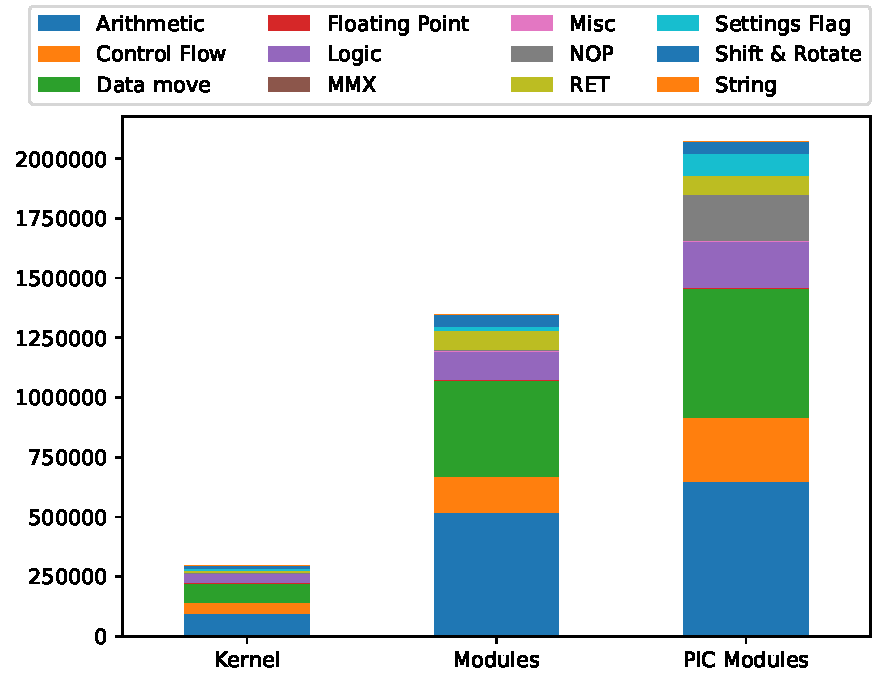
\includegraphics[width=0.6\columnwidth]{charts/gadget_distribution.pdf}
\caption{ROP Gadget Distribution}
\label{fig:gadget_dist}
\end{figure}

\subsubsection*{Gadget Quality}
To evaluate the quality of gadgets (second metric), we need to consider a concrete goal that an attacker might be interested in achieving. In our analysis, we consider the
\begin{lstlisting}
set_memory_x(unsigned long addr, int numpages)
\end{lstlisting}
function. This function is an attractive target for an attacker because by calling this function with appropriate arguments an attacker could disable the no-execute (NX) protection on memory pages of his choice. After disabling NX protection, any arbitrary code can be executed from target memory. In order to construct an ROP chain to disable the NX protection, the attacker first begins by targeting a particular memory address and then prepares the environment and function arguments. The ROP chain needs to contain instructions to perform the following operations:
\begin{enumerate}[noitemsep]
    \item Pivor Stack
    \item Load \verb|addr| argument into the register \verb|RDI|
    \item Load \verb|num_pages| argument into register \verb|RSI|
    \item Call \verb|set_memory_x|
\end{enumerate}

For all the available modules, we try to construct an ROP gadget to call the \verb|set_memory_x| function. Furthermore, we track if the ROP gadget has side-effects. The results are shown in Table~\ref{tbl:gadget_quality}. 80\% of the modules contain enough gadgets to form a ROP chain to disable NX protection.

\begin{table*}
    \caption{Gadget Categories}
    \begin{center}
    \begin{tabular}{lcc}
    \toprule
     & \textbf{Non-PIC} & \textbf{PIC} \\
    \midrule
    \textbf{Modules with ROP Chain, no side-effect} & 4,320 & 4,358 \\
    \textbf{Modules with ROP Chain, with side-effect} & 1 & 1 \\
    \textbf{Modules without ROP Chain} & 1,008 & 970 \\
    \hline
    \textbf{Total Number of Modules} & 5,329 & 5,329 \\
    \bottomrule
    \end{tabular}
    \end{center}
    \label{tbl:gadget_quality}
\end{table*}

From our evaluation, we found that Linux kernel modules contain 85\% of all the available gadgets. And 80\% of the modules contain enough gadgets to disable the NX protection without any side effects. Hence, re-randomization of the modules is a promising approach to mitigating the ROP attacks on Linux kernel.